\input{../include/preamble}

\title[ID1019 Higher order]{Higher order}


\author{Johan Montelius}
\institute{KTH}
\date{\semester}

\begin{document}

\begin{frame}
\titlepage
\end{frame}

\begin{frame}{let's play some cards}

\begin{columns}

 \begin{column}{0.2\linewidth}
   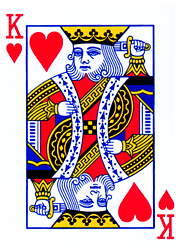
\includegraphics[width=\linewidth]{kung.png}
 \end{column}
 
 \pause

 \begin{column}{0.8\linewidth}
  \begin{itemize}
   \item ${\rm suit} \in \{{\rm :spade}, {\rm :heart}, {\rm :diamond}, {\rm :club}\}$
   \pause
   \item ${\rm value} \in \{2,3,\ldots 14\}$
   \pause 
   \item ${\rm card}$ = \{:card, suit, value\}
  \end{itemize}
 \end{column}
\end{columns}

\end{frame}

\begin{frame}[fragile]{order of cards}

\pause
\begin{verbatim}
lt({:card, s, v1}, {:card, s, v2})  do   v1 < v2 end
\end{verbatim}
\pause
\begin{verbatim}
lt({:card, :club, _}, _) do  true end
\end{verbatim}
\pause
\begin{verbatim}
lt({:card, :diamond, _}, {:card, :heart, _}) do true end
\end{verbatim}
\pause
\begin{verbatim}
lt({:card, :diamond, _}, {:card, :spade, _}) do true end
\end{verbatim}
\pause
\begin{verbatim}
lt({:card, :heart, _}, {:card, :spade, _}) do true end
\end{verbatim}
\pause
\begin{verbatim}
lt({:card, _, _}, {:card, _, _}) do false end
\end{verbatim}

\end{frame}

\begin{frame}[fragile]{sorting cards}

\begin{columns}

 \begin{column}{0.5\linewidth}
\begin{verbatim}
def sort([]) do [] end
\end{verbatim}
\pause
\begin{verbatim}
def sort(cards) do 
   {c1, c2} = split(cards)
   s1 = sort(c1)
   s2 = sort(c2)
   merge(s1, s2)
end
\end{verbatim}
 \end{column}
 
 \pause

 \begin{column}{0.5\linewidth}
\begin{verbatim}
def split([]) do
   {[], []}
end
\end{verbatim}
\pause
\begin{verbatim}
def split([c|s]) do
    {h1, h2} = split(s)
    {..., ...}
end
\end{verbatim}
 \end{column}
\end{columns}

\end{frame}

\begin{frame}[fragile]{tail recursive split}

\begin{columns}

 \begin{column}{0.5\linewidth}
\begin{verbatim}
def split([]) do
   {[], []}
end
\end{verbatim}
\pause
\begin{verbatim}
def split([c|s]) do
    {h1, h2} = split(s),
    {..., ...}
end
\end{verbatim}
 \end{column}
 
 \pause

 \begin{column}{0.5\linewidth}
\begin{verbatim}
def split(deck) do 
   split(deck, [], [])
end
\end{verbatim}

\pause
\begin{verbatim}
def split([], d1, d2) do
   {d1, d2}
end
\end{verbatim}
\pause
\begin{verbatim}
def split([c|s], d1, d2) do
   split(s, ..., ...)
end
\end{verbatim}
 \end{column}
\end{columns}

\end{frame}

\begin{frame}[fragile]{sorting cards}

\begin{verbatim}
def merge([], s2) do  ... end
def merge(s1, []) do  ... end
\end{verbatim}
\pause
\begin{verbatim}
def merge([c1|s1], [c2|s2]) do 
   case lt(c1, c2) of
     true ->
        [c1 | merge(s1, [c2|s2])]
     false ->
        [c2 | merge([c1|s1], s2)]
   end
end
\end{verbatim}

\end{frame}

\begin{frame}{what to do}

\pause Implement function that sorts names of people.

\pause Implement function that sorts a frequency table.

\pause Implement function that sorts ....


\end{frame}

\begin{frame}[fragile]{old friends}

Have we seen this before?

\pause\vspace{20pt}
\begin{columns}
   \begin{column}{.5\linewidth}
     \begin{block}{sum/1}
       \begin{verbatim}
def sum([]) do 0 end
def sum([h|t]) do
    add(h,sum(t))
end
       \end{verbatim}
       \vfill
     \end{block}
   \end{column} 
\pause
   \begin{column}{.5\linewidth}
     \begin{block}{prod/1}
       \begin{verbatim}
def prod([]) do 1 end
def prod([h|t]) do
   mul(h,prod(t))
end
       \end{verbatim}
       \vfill
     \end{block}
   \end{column}
  \end{columns}

\vspace{20pt}{\em There is no built-in add/2, nor mul/2, but we can pretend that there is.}

\end{frame}



\begin{frame}[fragile]{good to have}

We would like to to this:

\pause\vspace{20pt}

\begin{columns}
   \begin{column}{.5\linewidth}
     \begin{block}{foldr/3}
       \begin{verbatim}
def foldr([], acc, op) do
   acc
end
       \end{verbatim}
\pause
       \begin{verbatim}
def foldr([h|t], acc, op) do
   op.(h, foldr(t, acc, op))
end
      \end{verbatim}
       \vfill
     \end{block}
   \end{column}
\pause
   \begin{column}{.5\linewidth}
     \begin{block}{sum/1}
       \begin{verbatim}
def sum(l) do 
   add = ...,
   foldr(l, 0, add)
end
       \end{verbatim}
     \end{block}
\pause     
   \begin{block}{prod/1}
       \begin{verbatim}
def prod(l) do 
   mul = ...,
   foldr(l, 1, mul)
end
       \end{verbatim}
     \end{block}
   \end{column}
  \end{columns}

\pause\vspace{20pt}
{\em only problem, \ldots How do we express the function?}

\end{frame}

\begin{frame}[fragile]{lambda expressions}

We introduce a new data structure: a closure

  \vspace{20pt}

  \begin{tabular}{r l l}
   {\em Atoms} & = & \{a, b, c, \ldots\} \\
   {\em Closures} & = & \{f:e | f $\in $ Functions $\wedge$  e $\in $ Environment \}\\
   {\em Structures} & = & {\em Closures} $\cup$ {\em Atoms} $\cup$ \{ \{a, b\} \textbar a $\in$ {\em Structures}  $\wedge$  b $\in$ {\em Structures} \}
  \end{tabular}

\pause\vspace{10pt}
A {\em closure} is a function and an environment.

\pause\vspace{10pt}
We have not really defined what a {\em function} is nor an {\em environment} but let's forget this for a while.

\end{frame}

\begin{frame}[fragile]{function expressions}

\begin{code}
   <function> &::= 'fn' '(' <parameters> ')' '->' <sequence> 'end'\\
   <parameters> &::= '  ' | <variables> \\
   <variables> &::= <variable> |  <variable> ',' <variables>\\
\end{code}
\pause
\begin{code}
   <application> &::= <expression> '.' '(' <arguments> ')'\\
   <arguments> &::= '  ' | <expressions> \\
   <expressions> &::= <expression> |  <expression> ',' <expressions>\\
\end{code}
\pause
\begin{code}
   <expression> &::= <function> | <application> | ...\\
\end{code}

\end{frame}

\begin{frame}[fragile]{function expressions}

\pause\vspace{10pt}
We will write:
\pause\vspace{40pt}\hspace{60pt}\verb!x = 2; f = fn(y) -> {x,y} end; f.(4) !

\end{frame}


\begin{frame}[fragile]{evaluation of a function}

  \begin{itemize}
   \pause\item $E\sigma({\rm f})  \rightarrow  {\rm function}:\theta$ if
    \begin{itemize} 
           \pause\item $\mathrm{function}$ is the corresponding function of $f$
           \pause\item $\theta = \{ v/s \mid  v/s \in \sigma \wedge v {\rm\ free\  in\ f}\}$
    \end{itemize} 
  \end{itemize} 

\pause\vspace{20pt}

\begin{verbatim}
  x = 2; y = 3; z = 4; c = fn(v) -> v + y end; ...
\end{verbatim}

{\em What is C?}


\end{frame}

\begin{frame}[fragile]{evaluation of an application}

  \begin{itemize}
   \pause\item $E\sigma(e(e_1, \ldots)) \rightarrow E\{v_1/s_1, \ldots\}\cup\theta({\rm sequence} )$ if
    \begin{itemize}        
           \pause\item $E\sigma(e) \rightarrow f:\theta$
           \pause\item ${\rm f} = {\rm fun}(v_1, \ldots) \rightarrow  {\rm sequence}$ 
           \pause\item $E\sigma(e_i) \rightarrow s_i$ 
    \end{itemize} 
  \end{itemize}

\pause\vspace{20pt}

\begin{verbatim}
   y = 3; f = fn(v) -> v + y end; f.(4)
\end{verbatim}

\end{frame}
 
\begin{frame}[fragile]{example}

\begin{verbatim}
def foo(x) do
      y = 3
      fn(v) do v + y + x end
end
\end{verbatim}
\pause\vspace{20pt}

\begin{verbatim}
   f = foo(2); y = 7; f.(1)
\end{verbatim}
\end{frame}

\begin{frame}[fragile]{case closed}

\pause
     \begin{block}{sum/1}
       \begin{verbatim}
def sum(l) do
  add = fn(x,y) do x + y end
  foldr(l, 0, add)
end
       \end{verbatim}
     \end{block}
   \pause
     \begin{block}{prod/1}
       \begin{verbatim}
def prod(l) do 
  mul = fn(x,a) -> x * a end
  foldr(l, 1, mul)
end
       \end{verbatim}
\vfill
     \end{block}

\end{frame}

\begin{frame}[fragile]{example}

\pause What is gurka/1 doing?

\pause\vspace{20pt}

\begin{verbatim}
def gurka(l) do 
    d = fn(_, a) -> a + 1 end
    foldr(l, 0, f)
end
\end{verbatim}

\pause\vspace{20pt}
\pause How about tomat/1 doing?

\pause\vspace{10pt}
\begin{verbatim}
def tomat(l) do 
    f = fn(h, a) ->  a ++ [h] end
    foldr(l, [], f)
end
\end{verbatim}
\end{frame}

\begin{frame}[fragile]{example}
     \begin{block}{foldr/3}
       \begin{verbatim}
foldr([], acc, op) do  acc end
foldr([h|t], acc, op) do
   op.(h, foldr(t, acc, op))
end
       \end{verbatim}
       \vfill
     \end{block}
\pause

     \begin{block}{foldl/3}
       \begin{verbatim}
def foldl([], acc, op) do  acc end
def foldl([h|t], acc, op) do
   foldl(t, op.(h, acc), op)
end
       \end{verbatim}
     \end{block}
\end{frame}


\begin{frame}[fragile]{example}

\pause\vspace{10pt}
\begin{verbatim}
def tomat(l) -> 
    f = fn(h, a) ->  a ++ [h] end
    foldr(l, [], f)
end
\end{verbatim}
\pause 
\begin{verbatim}
def morot(l) do 
    f = fn(h, a) -> [h|a] end
    foldl(l, [], f)
end
\end{verbatim}
\end{frame}

\begin{frame}{left or right}

Which one should you use, {\em fold-left} or {\em fold-right}?

\end{frame}

\begin{frame}[fragile]{append all}

\pause Append all lists in a lists.

\vspace{20pt}

\begin{verbatim}
def appendl(l) do
    f = fn(e,a) -> a ++ e end,
    foldl(l, [], f)
end
\end{verbatim}

\begin{verbatim}
def appendr(l) do
    f = fn(e,a) -> e ++ a end
    foldr(L, [], F)
end
\end{verbatim}

\end{frame}



\begin{frame}{patterns}

In the {\tt List} module. 

\begin{itemize}
\item {\tt foldl(list, acc, fun)} : folds from the left 
\item {\tt foldl(list, acc, fun)} : folds from the left
\end{itemize}

\pause

In the {\tt Enum} module. 

\begin{itemize}
\item {\tt filter(enum, fun)}: return a list of all elements x, for which fun.(x) evaluates to true
\item {\tt map(enum, fun)}: return the list of fun.(x) for each element x in enum
\item {\tt sort(enum, fun)}: sort the enum given that the function is 'less than or equal'
\end{itemize}

\end{frame}

\begin{frame}[fragile]{Elixir shorthand}

\hspace{40pt}  {\tt fn(x,y) -> x + y + 5end}

\vspace{40pt}  \pause

\hspace{40pt}  {\tt \&(\&1 + \&2 + 5)}

\end{frame}


\begin{frame}[fragile]{an infinite list}

\pause\vspace{20pt}

\verb+inf = infinity()+\pause \verb+, [0|inf1] = inf()+\pause \verb+, [1|inf2] = inf1.()+

\pause
\begin{verbatim}
def infinity() do fun() -> infinity(0) end end
\end{verbatim}
\pause
\begin{verbatim}
def infinity(n) do [...|...] end
\end{verbatim}

\end{frame}


\begin{frame}[fragile]{the list of fibonacci }

A function that returns an infitie list of Fibonacci numbers.

\pause\vspace{20pt}

\begin{verbatim}
def fib() do fun() -> fib(1,1) end
\end{verbatim}
\pause
\begin{verbatim}
def fib(f1, f2) do [f1 | fn() -> fib(f2, f1+f2) end] end
\end{verbatim}

\pause\vspace{20pt}

\begin{verbatim}
> f0 = fib()

> [n0 | f1] = f0.()

> [n1 | f2] = f1.()
\end{verbatim}

\end{frame}

\begin{frame}{Higher order}

Order of what?

\pause\vspace{20pt}
A first order function takes a value, a data structures, as argument and returns a value.

\pause\vspace{20pt}
A second order function takes a first order function as argument or returns a first order function.

\pause\vspace{20pt}
A third order function ....

\pause\vspace{20pt}
Higher order functions takes a higher order ...

\pause\vspace{20pt}
Are functions considered to be ``first-class citizen''?
\end{frame}


\begin{frame}{not really}

\vspace{40pt}Not really - look at this.

\end{frame}

\begin{frame}{set comprehension}

In mathematics, {\em set comprehension}:

$$l = \lbrace 1,2,3,4,5,6,7,8 \rbrace ,  k = \lbrace 2*x | x \in l \wedge x < 5 \rbrace$$

\pause In functional programming, {\em list comprehension}:

\pause 
\vspace{20pt}\hspace{40pt} {\tt l = [1,2,3,4,5,6,7,8]; k = for n <- l, do: x*2 end}

\pause 
\vspace{20pt}\hspace{40pt} {\tt .. k = for n <- l, rem(n,2) == 0 do: n end}
\end{frame}


\begin{frame}[fragile]{quick sort}

\begin{verbatim}
  def qsort([]) do [] end
  def qsort([p|l]) do
    lower = for x <- l, x < p, do: x 
    higher = for x <- l, x >= p, do: x 
    qsort(lower) ++ [p | qsort(higher)]
  end
\end{verbatim}


\end{frame}


\begin{frame}{Summary}

\pause Higher order programming:

\begin{itemize}
\pause\item {closure}: a function and an environment
\pause\item {generic algorithms}: separate the recursive pattern from the data it operates over
\pause\item {continuations}: powerful technique to handle incomplete information
\pause\item {list comprehension}: very compact syntax for the construction of lists
\end{itemize}


\end{frame}


\end{document}



